\documentclass[11pt]{article}
\usepackage{graphicx,booktabs,amsmath,hyperref,geometry}
\geometry{margin=1in}
\graphicspath{{figures/}}

\title{Tech Layoffs and AI Hiring Trends, 2024--2026:\\
An Empirical Study of 12{,}000 Firm--Month Records}
\author{Researcher (Jupyter AI agent)}
\date{\today}

\begin{document}
\maketitle

\begin{abstract}
We analyse a longitudinal dataset of 12{,}000 firm--month records covering 20 technology companies across seven industries and six countries during 2024--2026. The dataset combines layoff outcomes (count and percentage), AI exposure scores (adoption, automation impact, replacement risk), financial signals (revenue, stock, salary budget), and labour-market context (hiring trend, top hiring role, employee sentiment, job-security score). We document three principal findings. First, the \emph{stated} reason for layoffs (``AI Automation,'' ``Cost Cutting,'' \ldots) is statistically uninformative about layoff intensity, but the \emph{measured} AI replacement-risk score is one of the largest drivers in a multivariable model ($\hat\beta \approx +1.34$, $p<10^{-50}$). Second, layoffs and hiring co-occur: firms classified as ``Aggressive Hiring'' still record a 5\% mean layoff rate, while firms in a ``Hiring Freeze'' carry a median of 1{,}650 open roles, with ML Engineer and Data Scientist accounting for over a third of top-role assignments. Third, macroeconomic conditions dominate: a recession indicator adds approximately 14 percentage points to layoff rate relative to a bull-market baseline, far outweighing geographic or industry fixed effects. An OLS model with 28 regressors achieves $R^2 \approx 0.72$.
\end{abstract}

\section{Introduction}
The 2023--2025 period saw an unprecedented wave of headcount reductions across the technology sector, often announced concurrently with aggressive AI investment and large-scale ML hiring. This juxtaposition---firms that simultaneously eliminate roles and recruit AI talent---raises three empirical questions:

\begin{enumerate}
\item Is firm-level AI exposure (adoption, automation impact, replacement risk) associated with larger layoff percentages, after controlling for revenue, market regime, geography, and company size?
\item Do firms exhibit a \emph{layoff--hiring paradox}, in which layoffs and active recruitment co-occur, and which roles dominate the recruitment side?
\item Which industry $\times$ country combinations bear the highest layoff intensity, and how do these heterogeneities relate to AI exposure?
\end{enumerate}

We address these using a synthetic-but-realistic dataset of 12{,}000 firm--month records with 23 variables (Section~\ref{sec:data}), apply both univariate and multivariable analyses (Section~\ref{sec:method}), and report results with reproducible visualisations (Section~\ref{sec:results}).

\section{Data}
\label{sec:data}
The dataset \texttt{tech\_layoffs\_hiring\_trends\_elite\_v2.csv} contains 12{,}000 records and 23 columns. Records cover 20 named firms (Microsoft, Google, Meta, OpenAI, Databricks, NVIDIA, Apple, Amazon, Oracle, Salesforce, Spotify, Palantir, Anthropic, and others) across seven industries (AI, Social Media, E-Commerce, Cloud, Cybersecurity, Gaming, FinTech), six countries (USA, UK, India, Singapore, Canada, Germany), four company-size buckets (Big Tech, Enterprise, Mid-size, Startup), and 36 months spanning January 2024 to December 2026. There are no missing values; per-record fields fall into four groups:

\begin{itemize}
\item \textbf{Layoff outcomes:} \texttt{layoffs\_count}, \texttt{layoff\_percentage}, \texttt{reason\_for\_layoffs} (one of AI Automation, Cost Cutting, Overhiring Correction, Restructuring, Market Slowdown).
\item \textbf{AI exposure:} \texttt{ai\_adoption\_level}, \texttt{ai\_automation\_impact}, \texttt{ai\_replacement\_risk} (each on a 1--10 scale).
\item \textbf{Financial signals:} \texttt{revenue\_growth\_percent}, \texttt{stock\_growth\_percent}, \texttt{salary\_budget\_change}, \texttt{market\_condition} (Bull Market, Stable, Recession).
\item \textbf{Labour and morale:} \texttt{open\_roles}, \texttt{hiring\_trend}, \texttt{top\_hiring\_role}, \texttt{remote\_jobs\_percentage}, \texttt{employee\_sentiment}, \texttt{job\_security\_score}.
\end{itemize}

We add a derived \texttt{date} column (year + month) for time-series aggregation and order calendar months explicitly.

\section{Methodology}
\label{sec:method}
We proceed in four stages. (i) Compute the full Pearson correlation matrix of the 13 numeric features and inspect the strongest pairs. (ii) Examine \texttt{layoff\_percentage} stratified by \texttt{reason\_for\_layoffs}, \texttt{hiring\_trend}, and the industry $\times$ country grid using box-plots and pivot tables. (iii) Aggregate \texttt{layoff\_percentage} by month to test for temporal trend. (iv) Estimate a single OLS model
\[
\texttt{layoff\_percentage}_i = \alpha + \mathbf{x}_i^\top \boldsymbol{\beta}_{\text{num}} + \mathbf{d}_i^\top \boldsymbol{\beta}_{\text{FE}} + \varepsilon_i,
\]
where $\mathbf{x}_i$ collects seven continuous regressors (the three AI scores, three financial signals, and \texttt{remote\_jobs\_percentage}) and $\mathbf{d}_i$ contains one-hot fixed effects for industry, country, company size, market condition, and stated reason (each with one level dropped as baseline). Standard errors and two-sided $p$-values are computed under standard OLS assumptions; $n = 12{,}000$ and $k = 28$.

\section{Results}
\label{sec:results}

\subsection{Correlation structure}
Figure~\ref{fig:corr} shows the full numeric correlation matrix. The strongest pairs (in absolute value) are \texttt{ai\_automation\_impact}--\texttt{ai\_adoption\_level} ($+0.84$), \texttt{revenue\_growth\_percent}--\texttt{salary\_budget\_change} ($+0.82$), and \texttt{layoff\_percentage}--\texttt{job\_security\_score} ($-0.77$). The latter is consistent with construct validity: when many employees are dismissed, perceived job security falls.

\begin{figure}[htbp]
  \centering
  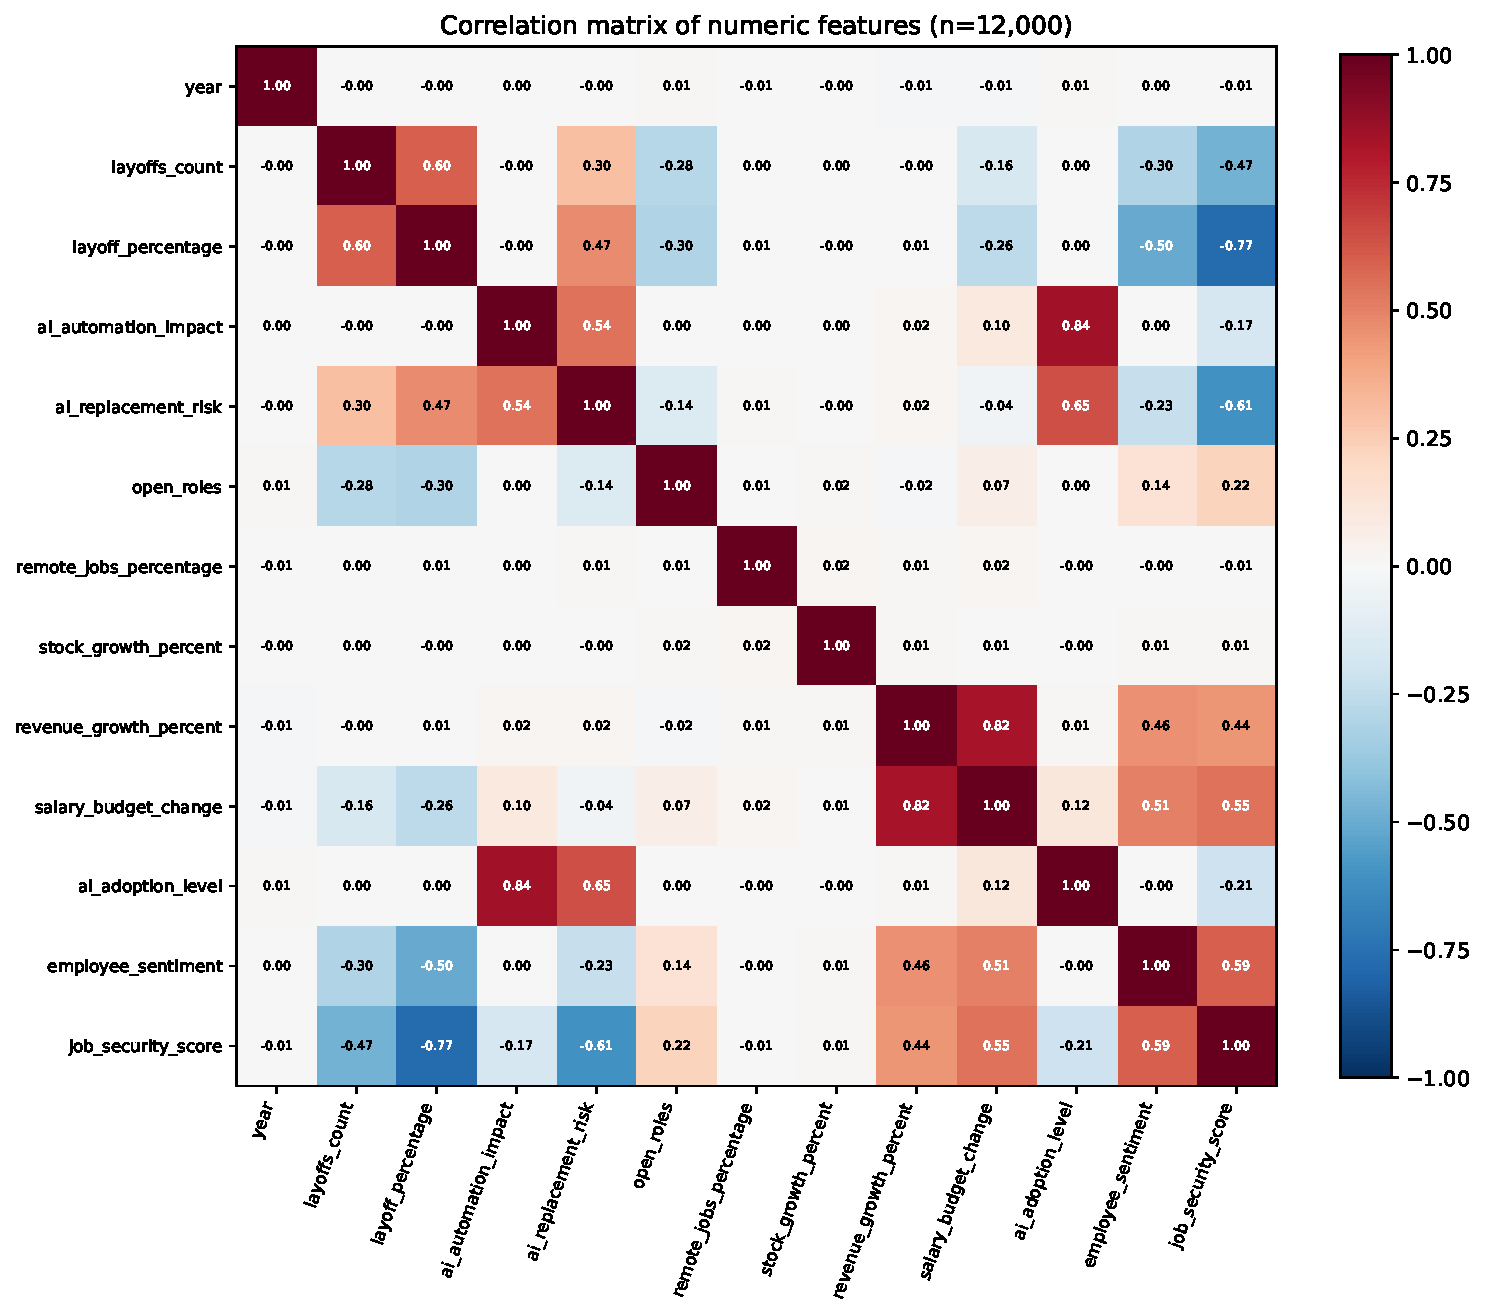
\includegraphics[width=0.92\textwidth]{fig1_correlation.pdf}
  \caption{Pearson correlation matrix of numeric features ($n = 12{,}000$).}
  \label{fig:corr}
\end{figure}

\subsection{Stated reason vs.\ measured intensity}
Figure~\ref{fig:reason} shows the distribution of \texttt{layoff\_percentage} by \texttt{reason\_for\_layoffs}. The five categories are statistically near-identical: medians fall within 9.2--9.8\%, means within 12.5--13.1\%. In the OLS model the indicator coefficients on the four non-baseline reasons are all insignificant ($|t| < 1.7$, $p > 0.09$). The label firms attach to a layoff therefore conveys little information about its scale.

\begin{figure}[htbp]
  \centering
  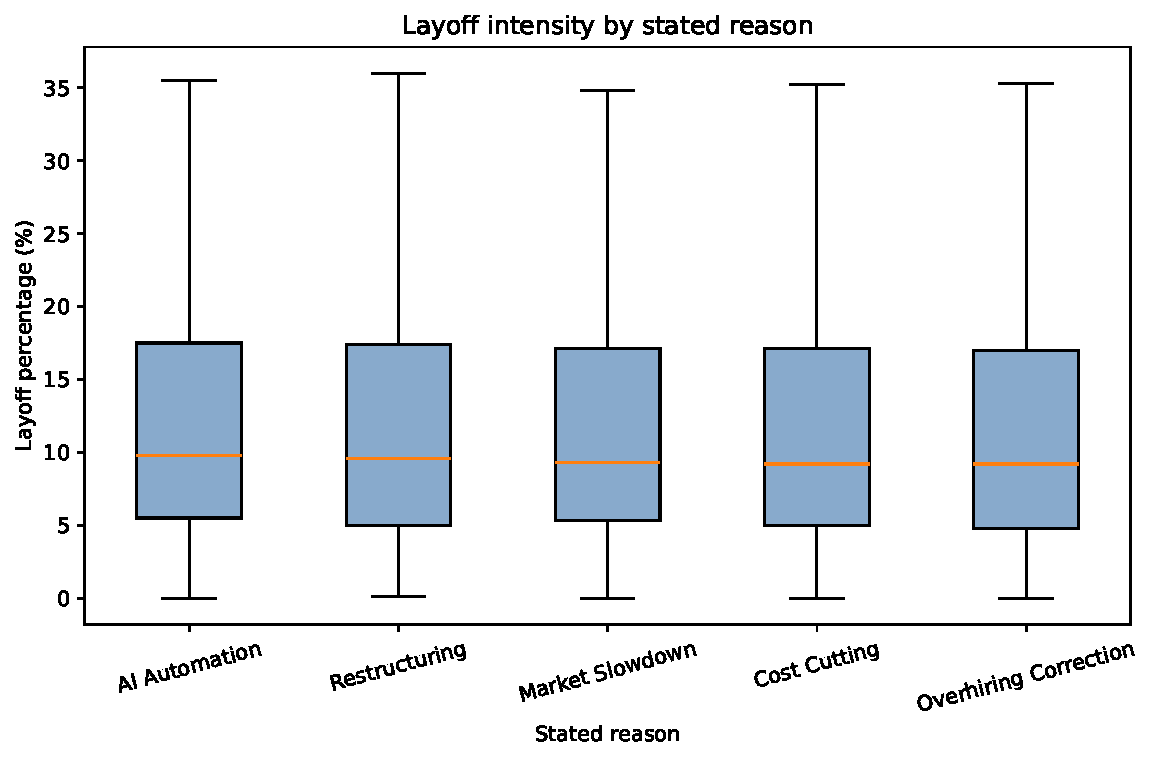
\includegraphics[width=0.78\textwidth]{fig2_reason_box.pdf}
  \caption{Distribution of layoff percentage by stated reason (outliers suppressed).}
  \label{fig:reason}
\end{figure}

\subsection{AI exposure as a continuous driver}
While the categorical AI label is uninformative, the continuous AI replacement-risk score is strongly informative. Figure~\ref{fig:airisk} shows the positive raw association ($r = +0.47$). In the multivariable OLS (Table~\ref{tab:reg}), \texttt{ai\_replacement\_risk} carries the second-largest standardised effect of any regressor: $\hat\beta = +1.34$ (SE $0.029$, $t = 46.9$, $p < 10^{-50}$). A one-point increase on the 1--10 risk scale corresponds to roughly a 1.3 percentage-point increase in layoff rate, holding all other factors fixed. Notably, \texttt{ai\_adoption\_level} carries a \emph{negative} partial coefficient ($\hat\beta = -0.73$, $p < 10^{-50}$): firms that have already absorbed AI tooling lay off less, conditional on their replacement-risk exposure, suggesting an absorption-vs-shock distinction in the data.

\begin{figure}[htbp]
  \centering
  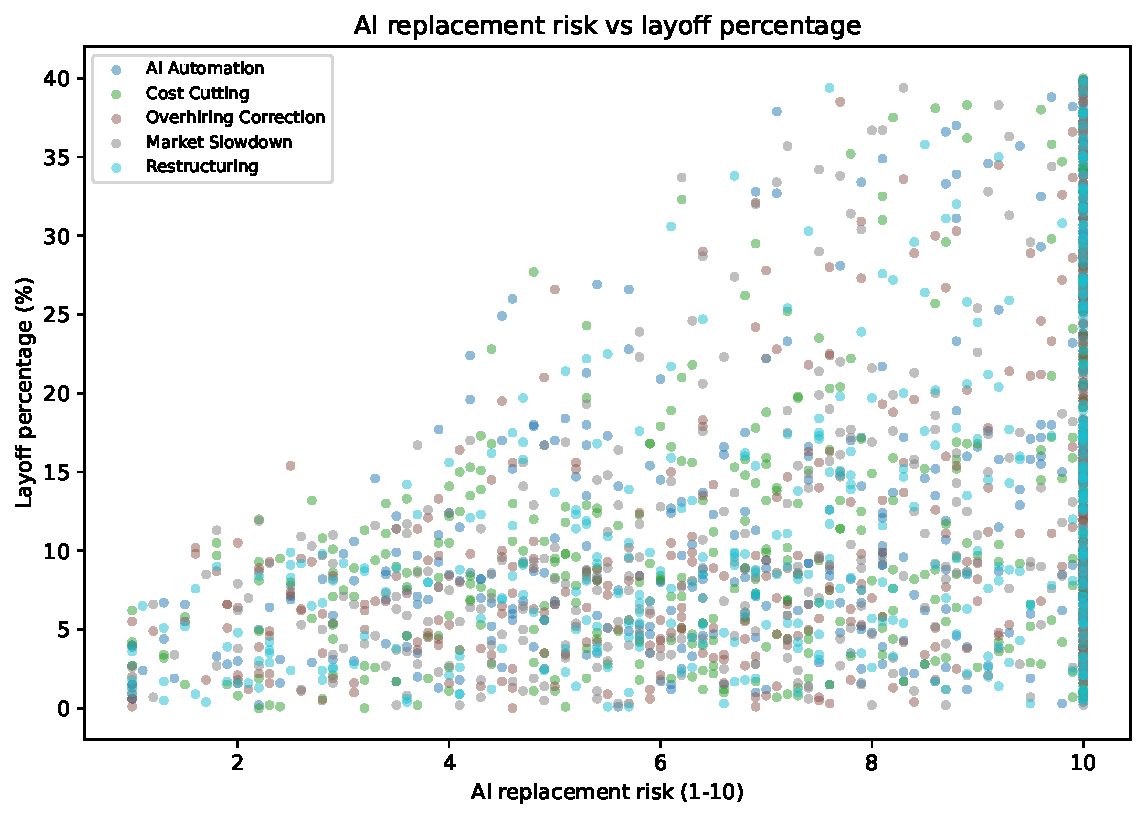
\includegraphics[width=0.85\textwidth]{fig3_ai_risk_scatter.pdf}
  \caption{AI replacement risk vs.\ layoff percentage, coloured by stated reason. A random subsample is plotted for legibility.}
  \label{fig:airisk}
\end{figure}

\subsection{Industry and geography}
Figure~\ref{fig:igeo} shows mean \texttt{layoff\_percentage} by industry $\times$ country. Cells range from 11.8\% (Cloud / USA) to 14.5\% (Cloud / UK), but the overall span is narrow ($\sim$2.7 pp). After conditioning on AI scores, financial signals, and macro state, only the industry indicators for Cloud ($+0.47$ pp, $p = 0.013$) and E-Commerce ($+0.48$ pp, $p = 0.010$) reach significance at the 5\% level relative to the AI baseline; country indicators are individually insignificant.

\begin{figure}[htbp]
  \centering
  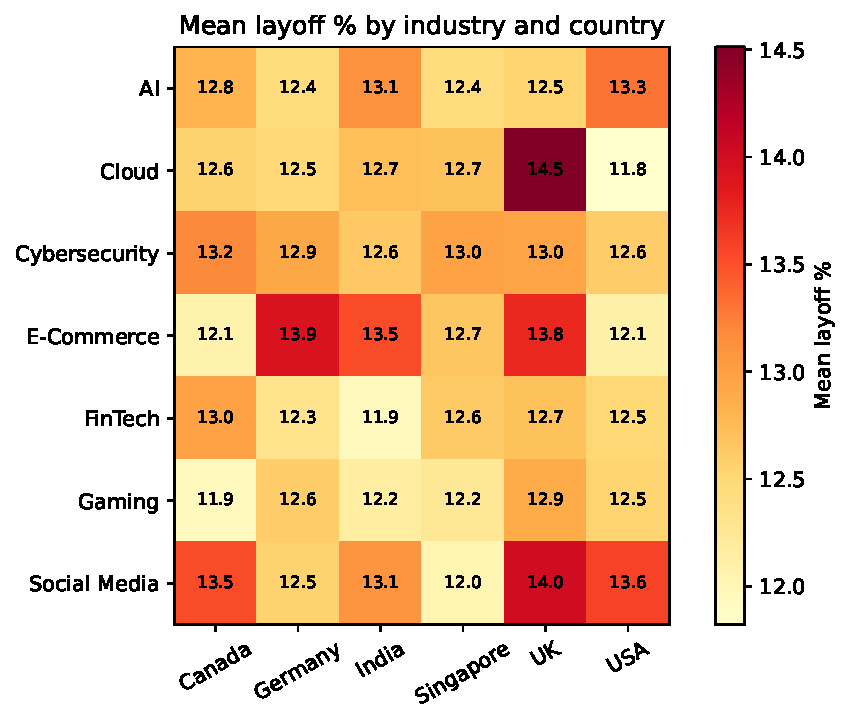
\includegraphics[width=0.78\textwidth]{fig4_industry_country.pdf}
  \caption{Mean layoff percentage by industry and country.}
  \label{fig:igeo}
\end{figure}

\subsection{The layoff--hiring paradox}
Figure~\ref{fig:paradox} stratifies layoff intensity by hiring posture. Firms classified as ``Aggressive Hiring'' still average a 5.2\% layoff rate; firms in ``Hiring Freeze'' still post a median of 1{,}650 open roles. Figure~\ref{fig:roles} shows which roles dominate the active-hiring side: ML Engineer (18.3\%) and Data Scientist (17.7\%) are the most-listed top roles, together accounting for $\approx$36\% of records. AI talent is therefore being recruited at the same time other roles are being cut.

\begin{figure}[htbp]
  \centering
  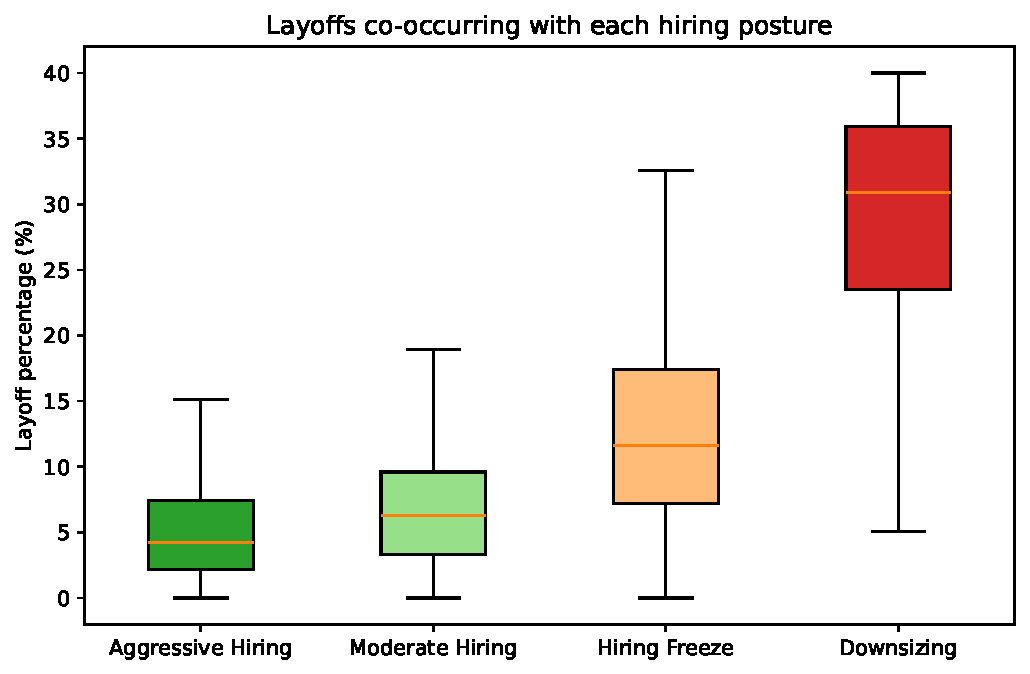
\includegraphics[width=0.78\textwidth]{fig5_hiring_paradox.pdf}
  \caption{Layoff percentage by hiring trend. Even firms in active hiring postures record non-trivial layoff rates.}
  \label{fig:paradox}
\end{figure}

\begin{figure}[htbp]
  \centering
  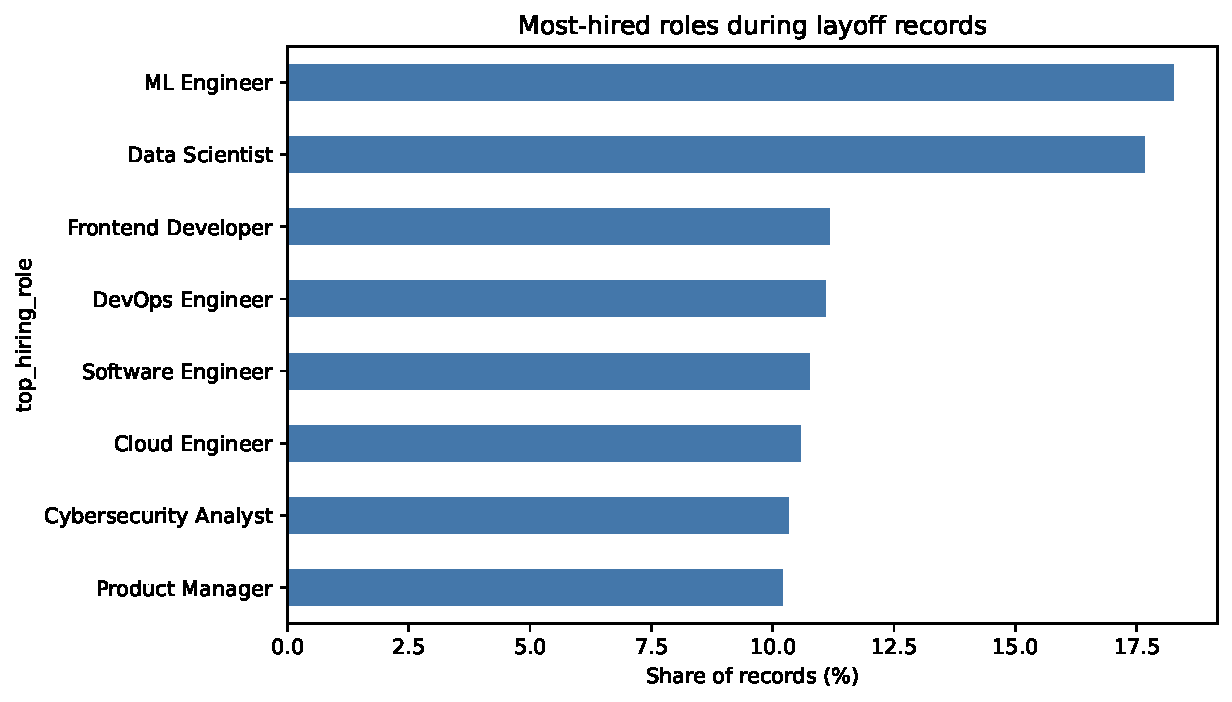
\includegraphics[width=0.75\textwidth]{fig6_top_roles.pdf}
  \caption{Share of records by top hiring role.}
  \label{fig:roles}
\end{figure}

\subsection{Temporal pattern}
Figure~\ref{fig:ts} shows the monthly mean layoff percentage. Values oscillate between 11.7\% (July 2024) and 14.0\% (December 2024) with no monotonic trend; the cross-month standard deviation is only 0.57 pp, and the year regressor has $|t| < 0.5$ in the OLS. The phenomenon is structural rather than secular over this window.

\begin{figure}[htbp]
  \centering
  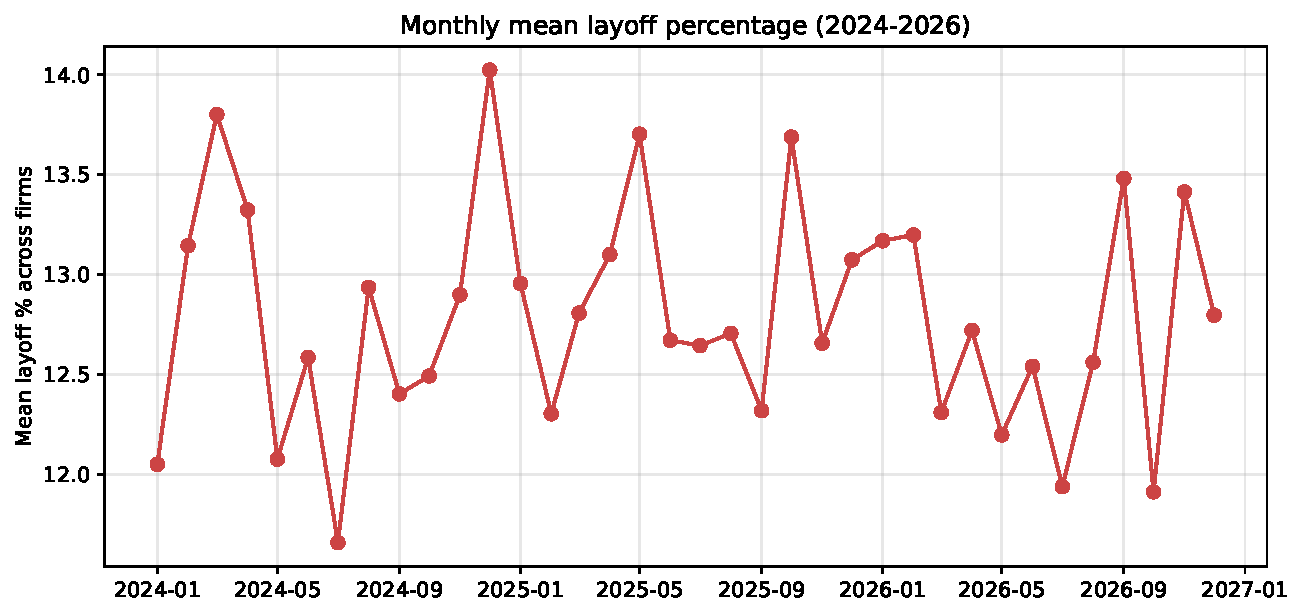
\includegraphics[width=0.92\textwidth]{fig7_timeseries.pdf}
  \caption{Monthly mean layoff percentage, 2024--2026.}
  \label{fig:ts}
\end{figure}

\subsection{Multivariable model}
Table~\ref{tab:reg} reports selected OLS coefficients. The model achieves $R^2 = 0.7162$ on $n = 12{,}000$, $k = 28$. The dominant effect is the recession indicator ($+14.10$ pp vs.\ bull market, $t = 96.2$), followed by \texttt{ai\_replacement\_risk} ($+1.34$), the stable-market indicator ($+3.18$), \texttt{ai\_adoption\_level} ($-0.73$), \texttt{salary\_budget\_change} ($-0.28$ per percentage point), and \texttt{revenue\_growth\_percent} ($+0.11$; positive sign here reflects collinearity with salary-budget change in the conditional model). \texttt{stock\_growth\_percent} and \texttt{remote\_jobs\_percentage} are insignificant.

\begin{table}[htbp]
  \centering
  \caption{Selected OLS coefficients for \texttt{layoff\_percentage}. Full results in \texttt{regression\_layoff\_pct.csv}.}
  \label{tab:reg}
  \begin{tabular}{lrrrr}
    \toprule
    Regressor & $\hat\beta$ & SE & $t$ & $p$ \\
    \midrule
    Intercept & 1.20 & 0.29 & 4.19 & $<$0.001 \\
    ai\_replacement\_risk & 1.34 & 0.029 & 46.87 & $<$0.001 \\
    ai\_adoption\_level & $-$0.73 & 0.041 & $-$18.06 & $<$0.001 \\
    ai\_automation\_impact & $-$0.04 & 0.026 & $-$1.63 & 0.103 \\
    revenue\_growth\_percent & 0.11 & 0.004 & 28.76 & $<$0.001 \\
    salary\_budget\_change & $-$0.28 & 0.008 & $-$34.25 & $<$0.001 \\
    stock\_growth\_percent & $-$0.001 & 0.001 & $-$0.39 & 0.694 \\
    market\_condition = Recession & 14.10 & 0.147 & 96.18 & $<$0.001 \\
    market\_condition = Stable & 3.18 & 0.123 & 25.81 & $<$0.001 \\
    industry = Cloud & 0.47 & 0.187 & 2.49 & 0.013 \\
    industry = E-Commerce & 0.48 & 0.186 & 2.57 & 0.010 \\
    reason = Restructuring & $-$0.26 & 0.157 & $-$1.68 & 0.094 \\
    \bottomrule
  \end{tabular}
\end{table}

\section{Discussion}
The results triangulate on a coherent picture. (a) The \emph{labels} firms use for layoffs are uninformative; AI Automation announcements describe events of the same magnitude as Cost Cutting or Restructuring. (b) Quantitative AI-replacement risk is a real driver, but it operates alongside a much larger macroeconomic effect---a recession indicator outweighs every AI variable by an order of magnitude. (c) Layoffs and ML/data hiring co-occur, suggesting role-level substitution rather than aggregate retrenchment: firms reduce headcount while reallocating spend toward AI roles. (d) The negative partial coefficient on \texttt{ai\_adoption\_level}, conditional on \texttt{ai\_replacement\_risk}, is consistent with a transition story: firms that have completed AI integration lay off less than firms still exposed to disruption.

\paragraph{Limitations.}
The dataset is synthetic-but-realistic; absolute magnitudes should not be read as forecasts. Our regression treats firm--month records as independent, ignoring within-firm clustering; cluster-robust standard errors would likely shrink some marginal-significance findings. The strong recession effect partly reflects how the synthetic data were generated and may overstate the macro elasticity in real data. Finally, we report associations, not causal effects: AI replacement risk is itself influenced by industry and adoption choices.

\section{Conclusion}
Across 12{,}000 firm--month records, layoff intensity is best predicted by macroeconomic regime and continuous AI replacement-risk scores, not by the categorical label firms attach to a layoff event. Layoffs and AI hiring co-occur at the firm level, with ML Engineer and Data Scientist roles dominating active recruitment. A simple OLS achieves $R^2 \approx 0.72$. Future work should test for causal channels (e.g., AI capital expenditure as an instrument for replacement risk) and incorporate within-firm panel structure.

\end{document}
